\documentclass[tikz,border=4pt]{standalone}
\begin{document}
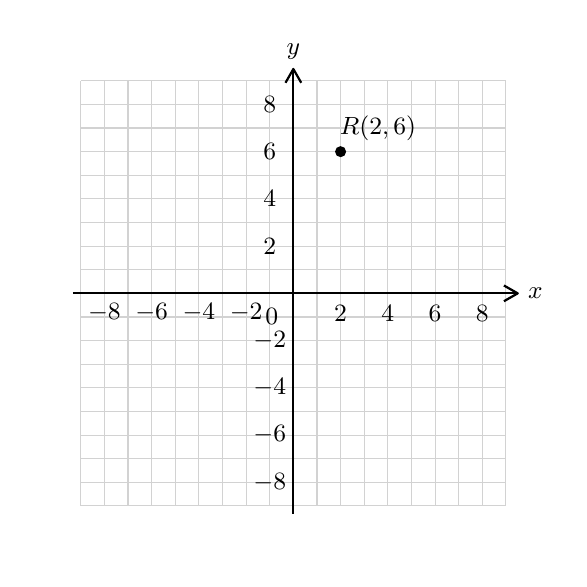
\begin{tikzpicture}[x=0.025cm,y=-0.025cm]
\path[use as bounding box] (0,0) rectangle (270,270);
\draw[gray!35,line width=0.4pt,line join=round] (27,27) -- (27,243);
\draw[gray!35,line width=0.4pt,line join=round] (27,27) -- (243,27);
\draw[gray!35,line width=0.4pt,line join=round] (39,27) -- (39,243);
\draw[gray!35,line width=0.4pt,line join=round] (27,39) -- (243,39);
\draw[gray!35,line width=0.4pt,line join=round] (51,27) -- (51,243);
\draw[gray!35,line width=0.4pt,line join=round] (27,51) -- (243,51);
\draw[gray!35,line width=0.4pt,line join=round] (63,27) -- (63,243);
\draw[gray!35,line width=0.4pt,line join=round] (27,63) -- (243,63);
\draw[gray!35,line width=0.4pt,line join=round] (75,27) -- (75,243);
\draw[gray!35,line width=0.4pt,line join=round] (27,75) -- (243,75);
\draw[gray!35,line width=0.4pt,line join=round] (87,27) -- (87,243);
\draw[gray!35,line width=0.4pt,line join=round] (27,87) -- (243,87);
\draw[gray!35,line width=0.4pt,line join=round] (99,27) -- (99,243);
\draw[gray!35,line width=0.4pt,line join=round] (27,99) -- (243,99);
\draw[gray!35,line width=0.4pt,line join=round] (111,27) -- (111,243);
\draw[gray!35,line width=0.4pt,line join=round] (27,111) -- (243,111);
\draw[gray!35,line width=0.4pt,line join=round] (123,27) -- (123,243);
\draw[gray!35,line width=0.4pt,line join=round] (27,123) -- (243,123);
\draw[gray!35,line width=0.4pt,line join=round] (135,27) -- (135,243);
\draw[gray!35,line width=0.4pt,line join=round] (27,135) -- (243,135);
\draw[gray!35,line width=0.4pt,line join=round] (147,27) -- (147,243);
\draw[gray!35,line width=0.4pt,line join=round] (27,147) -- (243,147);
\draw[gray!35,line width=0.4pt,line join=round] (159,27) -- (159,243);
\draw[gray!35,line width=0.4pt,line join=round] (27,159) -- (243,159);
\draw[gray!35,line width=0.4pt,line join=round] (171,27) -- (171,243);
\draw[gray!35,line width=0.4pt,line join=round] (27,171) -- (243,171);
\draw[gray!35,line width=0.4pt,line join=round] (183,27) -- (183,243);
\draw[gray!35,line width=0.4pt,line join=round] (27,183) -- (243,183);
\draw[gray!35,line width=0.4pt,line join=round] (195,27) -- (195,243);
\draw[gray!35,line width=0.4pt,line join=round] (27,195) -- (243,195);
\draw[gray!35,line width=0.4pt,line join=round] (207,27) -- (207,243);
\draw[gray!35,line width=0.4pt,line join=round] (27,207) -- (243,207);
\draw[gray!35,line width=0.4pt,line join=round] (219,27) -- (219,243);
\draw[gray!35,line width=0.4pt,line join=round] (27,219) -- (243,219);
\draw[gray!35,line width=0.4pt,line join=round] (231,27) -- (231,243);
\draw[gray!35,line width=0.4pt,line join=round] (27,231) -- (243,231);
\draw[gray!35,line width=0.4pt,line join=round] (243,27) -- (243,243);
\draw[gray!35,line width=0.4pt,line join=round] (27,243) -- (243,243);
\draw[black,line width=0.8pt,line join=round] (23,135) -- (249,135);
\draw[black,line width=0.8pt,line join=round] (135,247) -- (135,21);
\draw[black,line width=0.8pt,line join=round] (242,131) -- (249,135) -- (242,139);
\draw[black,line width=0.8pt,line join=round] (131,28) -- (135,21) -- (139,28);
\node[font=\small,inner sep=0pt] at (39,145) {$-8$};
\node[font=\small,inner sep=0pt] at (123,231) {$-8$};
\node[font=\small,inner sep=0pt] at (63,145) {$-6$};
\node[font=\small,inner sep=0pt] at (123,207) {$-6$};
\node[font=\small,inner sep=0pt] at (87,145) {$-4$};
\node[font=\small,inner sep=0pt] at (123,183) {$-4$};
\node[font=\small,inner sep=0pt] at (111,145) {$-2$};
\node[font=\small,inner sep=0pt] at (123,159) {$-2$};
\node[font=\small,inner sep=0pt] at (159,145) {$2$};
\node[font=\small,inner sep=0pt] at (123,111) {$2$};
\node[font=\small,inner sep=0pt] at (183,145) {$4$};
\node[font=\small,inner sep=0pt] at (123,87) {$4$};
\node[font=\small,inner sep=0pt] at (207,145) {$6$};
\node[font=\small,inner sep=0pt] at (123,63) {$6$};
\node[font=\small,inner sep=0pt] at (231,145) {$8$};
\node[font=\small,inner sep=0pt] at (123,39) {$8$};
\node[font=\small,inner sep=0pt] at (124,147) {$0$};
\node[font=\small,inner sep=0pt] at (258,135) {$x$};
\node[font=\small,inner sep=0pt] at (135,12) {$y$};
\fill (159,63) circle[radius=2pt];
\node[font=\small,inner sep=0pt] at (178,51) {$R(2,6)$};
\end{tikzpicture}
\end{document}
